\section{Phase 4: Training \& Evaluation}

\subsection{Validation Strategy}
The cleaned dataset (24,967 products) was split once into \textbf{70\% train / 15\% validation / 15\% test} (17,476 / 3,745 / 3,746 products; \texttt{split\_data.py}), \textbf{stratified by product category} with a fixed seed (42), so that rare categories such as footwear and outerwear appear in every split. The training set fits the weights, the validation set is used for hyperparameter selection, and the test set (\testN\ products) is used \emph{once} for the final numbers. K-fold cross-validation was not used because the sentence embeddings are frozen and the dataset is large, so a single stratified hold-out gives stable estimates at a fraction of the cost.

\subsection{Training Behaviour}
\begin{figure}[htbp]
\centering
\IfFileExists{../figures/mlp_loss_curve.png}{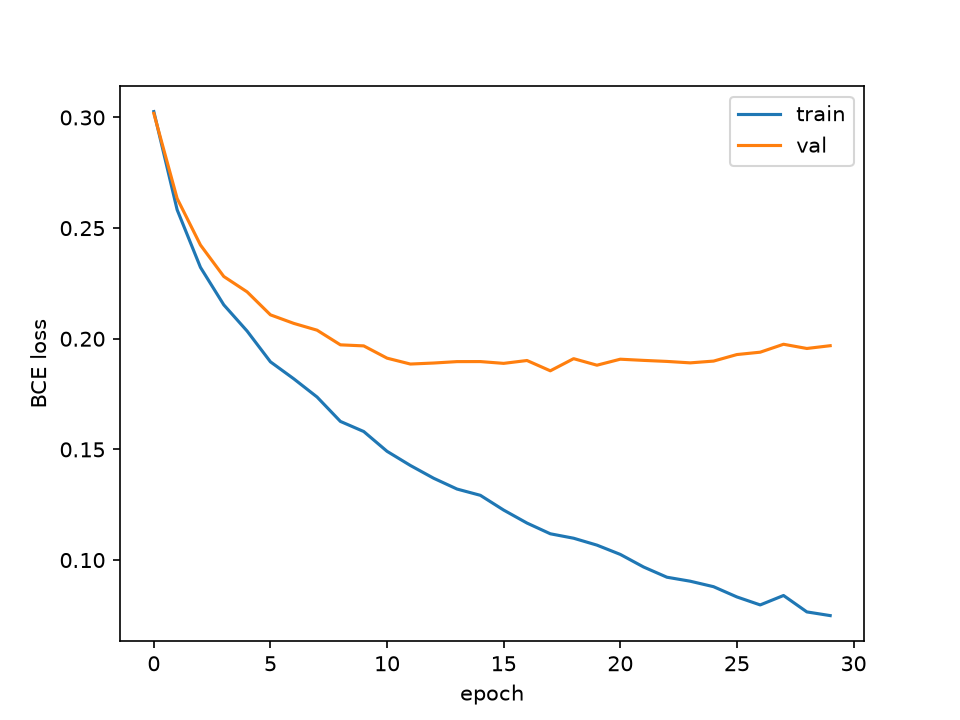
\includegraphics[width=0.7\linewidth]{../figures/mlp_loss_curve.png}}{\textbf{[missing]}}
\caption{Training and validation BCE loss of the selected model.}
\label{fig:loss}
\end{figure}
Figure~\ref{fig:loss} shows the binary cross-entropy loss per epoch. Both curves fall quickly from about 0.30 during the first ten epochs. The validation loss then flattens at about 0.19 and even rises slightly after epoch 25, while the training loss keeps decreasing to about 0.075. The growing gap shows that the network begins to overfit after roughly ten epochs. Since the weights of the last epoch are saved, early stopping (keeping the epoch with the lowest validation loss) would be a simple improvement; the gap is moderate and the test results below show that generalization is still good.

\subsection{Metrics and Why They Fit This Problem}
Plain accuracy is not informative for a multi-label task: each product has five yes/no decisions, and the labels are unevenly distributed (casual 68.7\%, presentation 53.9\%, office 53.8\%, concert 43.1\%, wedding 42.1\% of the test set), so a model leaning on the frequent labels would still score well on accuracy alone. We therefore report:
\begin{itemize}
  \item \textbf{Precision} -- of the products the model assigns to an occasion, how many truly belong. Low precision means the outfit builder would recommend unsuitable items.
  \item \textbf{Recall} -- of the products that suit an occasion, how many are found. Low recall shrinks the choice of items.
  \item \textbf{F1-score} -- harmonic mean of the two; we use the \emph{macro} average so rare occasions count as much as common ones.
  \item \textbf{AUC-ROC} -- threshold-independent ranking quality of the probabilities, useful because the 0.5 threshold is not tuned.
  \item \textbf{Exact match and Hamming loss} -- strict (all five labels right) and per-label error rates for the multi-label setting.
\end{itemize}

\subsection{Results on the Test Set}
\begin{table}[htbp]
\centering
\begin{tabular}{lcccc}
\toprule
Model & Precision & Recall & F1 & AUC-ROC \\
\midrule
Logistic regression (validation) & \baseP & \baseR & \baseF & \baseA \\
MLP, selected (validation) & 0.933 & 0.918 & \bestValF & \bestValAUC \\
\textbf{MLP, selected (test)} & \testPrec & \testRec & \testFone & \testAUC \\
\bottomrule
\end{tabular}
\caption{Macro-averaged metrics. Test micro-F1 is \testMicroF, Hamming loss \testHamming\ and exact-match ratio \testExact.}
\end{table}

The neural network clearly outperforms the logistic-regression baseline on the same validation data: macro F1 rises from \baseF\ to \bestValF\ and AUC-ROC from \baseA\ to \bestValAUC. The gain comes from both precision (0.896 against 0.933) and recall (\baseR\ against 0.918), so the non-linear hidden layers separate the occasions better than a linear model on the same embeddings. The test-set scores (F1 \testFone, AUC-ROC \testAUC) are about the same as the validation scores, so the model has not overfit the validation set through hyperparameter selection.

\begin{table}[htbp]
\centering
\IfFileExists{tables/per_class.tex}{\begin{tabular}{lrrrrrrrr}
\toprule
Class & Support & Prevalence & Precision & Recall & F1 & AUC & FP & FN \\
\midrule
casual & 2574 & 0.687 & 0.924 & 0.916 & 0.920 & 0.959 & 195 & 216 \\
concert & 1616 & 0.431 & 0.921 & 0.914 & 0.917 & 0.983 & 127 & 139 \\
office & 2014 & 0.538 & 0.940 & 0.938 & 0.939 & 0.985 & 120 & 125 \\
presentation & 2018 & 0.539 & 0.941 & 0.942 & 0.941 & 0.987 & 120 & 117 \\
wedding & 1577 & 0.421 & 0.940 & 0.906 & 0.923 & 0.983 & 91 & 148 \\
\bottomrule
\end{tabular}
}{\textbf{[run src/error\_analysis.py]}}
\caption{Per-class test results (FP/FN = false positives / false negatives).}
\label{tab:perclass}
\end{table}

\safefig{roc_per_class}{Per-class ROC curves on the test set.}

\subsection{Error Analysis}
\safefig{confusion_per_class}{Binary confusion matrix of each occasion label on the test set.}

Overall the model reaches a macro F1 of \testFone\ and an AUC-ROC of \testAUC\ on the test set, and 932 of the 3,746 test products (24.9\%) have at least one wrong label. The five classes perform very similarly (Table~\ref{tab:perclass}): F1 ranges only from 0.917 (concert) to 0.941 (presentation). Errors are balanced between false positives and false negatives. \emph{Casual} produces the most mistakes in absolute terms (195 false positives and 216 false negatives), partly because it is the most frequent label and has the lowest AUC (0.959); its definition is also the most vague, since it is the fallback label for products that match no other keyword rule. \emph{Wedding} has the lowest recall (0.906, 148 false negatives), which means some wedding products are missed, while its precision is high (0.940).

\emph{Office} and \emph{presentation} obtain the best scores (F1 0.939 and 0.941), but this should not be read as a deeper understanding of formal wear. As noted in Phase 2, these two labels come from almost identical keyword lists, so they are nearly the same label, and in interactive tests the model predicted them together (for example, ``formal blazer'' scored 1.00 for both). The very high scores also reflect that the labels are derived by keyword rules from the same product text: the network mainly learns to reproduce those rules, so some of the remaining errors are caused by noisy labels (for example ``blazer'' was also predicted as casual with probability 0.90) rather than by the model.

Table~\ref{tab:errors} lists the most confident mistakes. Many involve products whose title contains a keyword that conflicts with the description, or labels produced by broad keyword rules (e.g.\ ``embroidered'' $\to$ wedding), which means part of the ``error'' is noise in the heuristic labels rather than a model failure.
\begin{table}[htbp]
\centering
\small
\IfFileExists{tables/errors.tex}{\begin{tabular}{p{3.6cm}p{2.2cm}p{4.2cm}p{4.2cm}}
\toprule
Product title & Brand & True labels & Predicted \\
\midrule
EARRINGS (E2840/111/131) & Ethnc & concert & casual, office, presentation \\
CHUNKY SLIDES & Lama & concert & casual, concert \\
White Cotton Shalwar (MPS25S & Bonanza Satr & casual, wedding & casual \\
Regil Long & Lulusar & casual & casual, concert, office, presentation \\
SHIRT (E0750/119/112) & Ethnc & wedding & office, presentation, wedding \\
SKIRT (E3602/108/901) & Ethnc & office, presentation & office, presentation, wedding \\
Bella - 3 PC (WSS25P3024) & Bonanza Satr & concert, office, presentation, wedding & casual, concert, office, presentation \\
BROWN TRENDY PESHAWARI SANDA & J. & casual, wedding & casual \\
\bottomrule
\end{tabular}
}{\textbf{[run src/error\_analysis.py]}}
\caption{Most confident errors on the test set.}
\label{tab:errors}
\end{table}

\subsection{Bias Check}
The project aims at inclusive recommendations, so we checked whether performance differs across groups. Skin-tone and body-type labels do not exist in the data yet (Phase 2), so \textbf{brand, gender, category and plus-size availability} are used as available proxies: if the model works much worse for a group, products from that group (e.g.\ women's wear, plus-size items, small brands) would receive worse recommendations.

\safefig{bias_check}{Macro F1 per subgroup on the test set (groups with fewer than 30 products are skipped).}
\begin{table}[htbp]
\centering
\small
\IfFileExists{tables/bias.tex}{\begin{tabular}{llrrr}
\toprule
Attribute & Group & n & Macro F1 & Gap vs overall \\
\midrule
brand & Lama & 68 & 0.695 & -0.233 \\
brand & Lulusar & 407 & 0.765 & -0.163 \\
brand & Ethnc & 446 & 0.867 & -0.061 \\
brand & Hussain Rehar & 36 & 0.928 & -0.000 \\
brand & J. & 1255 & 0.953 & 0.025 \\
brand & Bonanza Satrangi & 1356 & 0.956 & 0.028 \\
brand & Outfitters & 149 & 0.971 & 0.043 \\
category & top & 764 & 0.855 & -0.073 \\
category & accessory & 345 & 0.860 & -0.068 \\
category & footwear & 119 & 0.875 & -0.053 \\
category & bottom & 538 & 0.878 & -0.050 \\
category & outerwear & 77 & 0.893 & -0.035 \\
category & set & 1903 & 0.957 & 0.029 \\
gender & unisex & 771 & 0.879 & -0.049 \\
gender & women & 2130 & 0.943 & 0.015 \\
gender & men & 845 & 0.950 & 0.022 \\
has\_plus\_sizes & 1 & 677 & 0.919 & -0.009 \\
has\_plus\_sizes & 0 & 3069 & 0.930 & 0.002 \\
\bottomrule
\end{tabular}
}{\textbf{[run src/plot\_results.py]}}
\caption{Subgroup macro F1 and gap to the overall test F1.}
\end{table}

Overall test macro F1 is \testFone. Performance is very similar for plus-size and other products (0.919 for products offering 2XL or larger, 0.930 for the rest, a gap of 0.011), so we found no meaningful disadvantage for plus-size items. Gender differences are small for men (0.950) and women (0.943), but \emph{unisex} products score lower (0.879).

The largest differences appear across \textbf{brands} and \textbf{categories}. Among brands, F1 ranges from 0.971 (Outfitters) and 0.956 (Bonanza Satrangi) down to 0.867 (Ethnc), 0.765 (Lulusar) and 0.695 (Lama), a spread of 0.276. Lama has only 68 test products, so its estimate is noisy, but Lulusar (407 products) is a reliable signal that the model is clearly worse on this brand, 0.163 below the overall score. Among categories, sets score highest (0.957) while tops (0.855), accessories (0.860) and bottoms (0.878) are 5 to 7 points below the average. A likely reason is that the dataset is dominated by a few brands and by sets (50.8\% of all products), so the model sees much more of their vocabulary and style of description, while other brands and single garments use different wording; we did not test this explanation directly. In the final application, recommendations for the weaker brands and categories (and for unisex items) would therefore be less reliable, so the occasion check should be treated with more caution for them. Possible remedies are oversampling weak groups, brand-balanced training and evaluation, and manual label checks on the weak subgroups.

\paragraph{Limitations.} (i) The labels are keyword heuristics derived from the same text the model reads, so high scores partly measure how well the network reproduces our rules, not real shopper opinion; (ii) the data comes from two dominant brands (68.7\% of products); (iii) no real demographic attributes are available, so the bias check cannot assess skin tone or body type directly; (iv) the threshold of 0.5 is the same for all labels; (v) the final epoch rather than the best epoch is saved. Future work: manual labels for a sample, per-class thresholds, early stopping, and fine-tuning the encoder.